
\documentclass[a4paper,11pt]{article}
\usepackage[utf8]{inputenc}
\usepackage[T1]{fontenc}
\usepackage[frenchb]{babel}

\usepackage{graphicx}
\usepackage{fancyhdr}
\usepackage{geometry}

\usepackage[colorlinks,linkcolor=blue]{hyperref}
\usepackage{amsmath}
\usepackage{amssymb}
\usepackage{mathrsfs}
\usepackage{epsfig}
\usepackage {eurosym}

\usepackage{float}

\geometry{a4paper,tmargin=2cm,bmargin=2cm,lmargin=1.5cm,rmargin=1cm,headheight=2.2cm,headsep=0.5cm,footskip=1cm}
\columnsep=0.6cm

\graphicspath{{images/}} 

\usepackage{listings}
\usepackage{color}
\usepackage{xcolor}

\usepackage{tikz}
\usepackage[siunitx]{circuitikz}


\lstset{columns=flexible,keepspaces=true, breaklines,breakindent=0pt} 


\lstset{language=C++,
basicstyle=\ttfamily\footnotesize,
breaklines, 
keywordstyle=\bfseries\color{blue},
stringstyle=\color{red},
commentstyle=\color{blue!20!black!30!green},
morecomment=[s][\color{black}]{/**}{*/},
numbers=left,
numberstyle=\tiny\color{black},
stepnumber=2,
numbersep=10pt,
tabsize=4,
showspaces=false,
showstringspaces=false}


\fancypagestyle{plain}{
% noms des respo   dans le bas de page                                            
\lfoot{Projet de C++}
\rfoot{M.Morin J.Fourmann}
\renewcommand{\headrulewidth}{0pt}
\fancyhead{}}
% Titre a compl»ter
\title{\textbf{ \huge{Projet de programmation C++}} \\{\Large  Résolution de circuit}}

\author{
\textsc{Jérémie Fourmann} (Promo 2013 - Eléctronique - Enseeiht)\\ %mettre votre nom
\textsc{Maxime Morin} (Promo 2013 - Eléctronique - Enseeiht)\\ %mettre votre nom
%\textsc{ddd dddd} (Promo - departement - respo)     %2 nom
}

\graphicspath{{images/}}

\begin{document}

\pagestyle{plain}

\maketitle
\vspace{1cm}
\renewcommand{\contentsname}{Plan}
\tableofcontents
\vspace{2cm}



\newpage


%Objectif

\section{Objectif}
\section{Organistion du code}
  \subsection{L'objet circuit}
    \begin{figure}[H]
	 \begin{center}
	  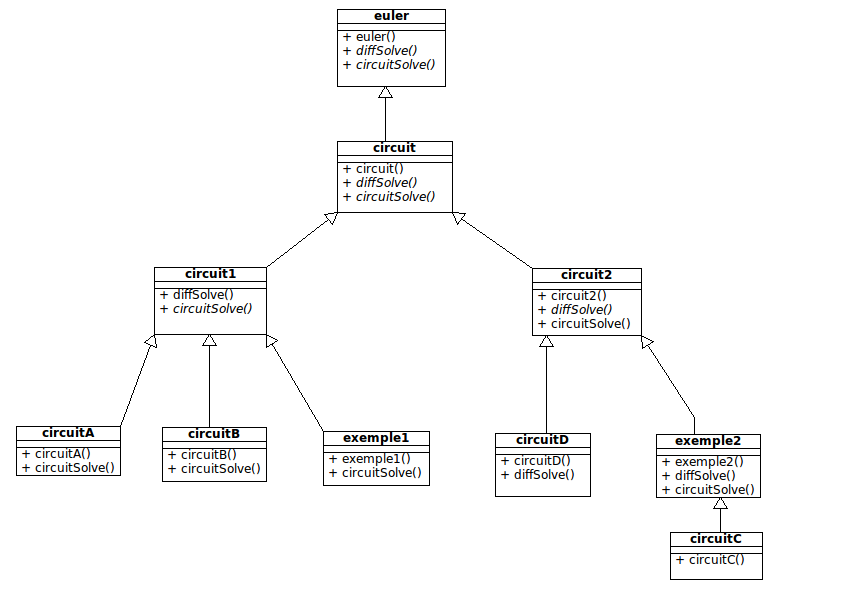
\includegraphics[scale=.7]{circuitDiagram}
	\caption{Hièrarchie de la classe circuit}
	\end{center}
      \end{figure}

  \subsection{L'objet source}
    \begin{figure}[H]
	 \begin{center}
	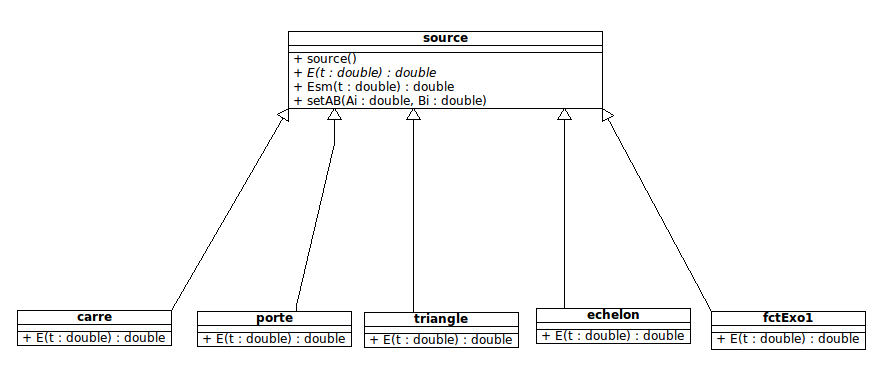
\includegraphics[scale=.7]{sourceDiagram}
	\caption{Hièrarchie de la classe source}
	\end{center}
      \end{figure}
\newpage


\section{Résultats}
  \subsection{Réponse du l'exemple 1}
  \subsection{Réponses du CircuitA}

\begin{circuitikz} \draw
 (1.5,0) node[ground] {}
  (0,0) to [V, v=$E(t)$, <->,>=latex] (0,3) to [R, l=$R$] (3,3)
  to [C, l=$C$, *-*] (3,0)
 (3,0) -- (0,0)
;\end{circuitikz}

\begin{circuitikz} \draw
 (0,0) node[anchor=east]{B}
  to[short, o-*] (1,0)
  to[R, l=$20\ohm$, *-*] (1,2)
  to [R, v=$v_x$, l=$10\ohm$] (3,2)
  to[short] (4,2) to[cI, i=$\frac{\siemens}{5}v_x$, *-*] (4,0)
   to[short] (3,0) to[R, l=$5\ohm$, *-*] (3,2)
 (3,0) -- (1,0)
 (1,2) to[short, *-o] (0,2)
  node[anchor=east]{A}
;\end{circuitikz}

\begin{circuitikz} \draw
 (0,0) to[C, l=$10\micro\farad$] (0,2) -- (0,3)
  to[R, l=$2.2\kilo\ohm$] (4,3) -- (4,2)
  to[L, l=$12\milli\henry$, i=$i_1$] (4,0) -- (0,0)
 (4,2) to[D*, *-*] (2,0) to [D*, -*] (0,2)
  to[R, l=$1\kilo\ohm$] (2,2)   to[cV, v=$0.3\kilo\ohm i_1$] (4,2)
 (2,0) to[I, i=$1\milli\ampere$:15, -*] (2,2)
; \end{circuitikz} 

  \subsection{Réponse du CircuitB}
 
   
    
  \subsection{Réponse du CircuitC}
  \subsection{Réponse du CircuitD}

  \appendix
  \newpage
  \section{main.cpp}
    \lstinputlisting{../main.cpp}
    \newpage
  \section{circuits.h}
    \lstinputlisting{../circuits.h}
    \newpage
  \section{circuits.cpp}
    \lstinputlisting{../circuits.cpp}
    \newpage
   \section{sources.h}
    \lstinputlisting{../sources.h}
    \newpage
   \section{sources.cpp}
    \lstinputlisting{../sources.cpp}
    \newpage

\end{document}
